\documentclass[8pt,landscape,a4paper]{extarticle}
\usepackage[margin=0.5cm]{geometry}
\usepackage{titlesec,fancyhdr,subcaption,amsmath,amsfonts,amsthm,amssymb,xcolor,ragged2e,graphicx}
\usepackage[bookmarksopen=true]{hyperref}
\usepackage{newpxtext,newpxmath,changepage,marginnote,mathtools,multicol,etoolbox,tcolorbox,pgf}
\usepackage[utf8]{inputenc}
\usepackage{tabularx}

\usepackage{enumitem}

\setlist[enumerate]{itemsep=0pt, parsep=0pt, topsep=0pt, partopsep=0pt}

\usepackage[citestyle=alphabetic,bibstyle=authortitle]{biblatex}
\addbibresource{references.bib}

\usepackage{amsmath} % Add this line to import the amsmath package
% ------ MDP Stuff ------ %
\newcommand{\states}{\mathcal{S}}
\newcommand{\nstates}{\lvert\states\rvert}
\newcommand{\actions}{\mathcal{A}}
\newcommand{\nactions}{\lvert\actions\rvert}
\newcommand{\timehorizon}{\mathcal{T}}
\newcommand{\localNumStates}{n_{\text{loc}}}


% ------ Math Stuff ------ %
\DeclareMathOperator*{\ev}{\mathbb{E}}
\DeclareMathOperator*{\Prob}{\mathbb{P}}
\newcommand{\R}{\mathbb{R}}
\newcommand{\N}{\mathbb{N}}
\newcommand{\E}{\mathbb{E}}
\newcommand{\bigO}{\mathcal{O}}
\newcommand{\jac}{\mathcal{J}}
\newcommand{\K}{\mathcal{K}} % Krylov subspace
\newcommand{\Lspace}{\mathcal{L}} % other subspace for KSP

\DeclareMathOperator*{\argmax}{arg\,max}
\DeclareMathOperator*{\argmin}{arg\,min}


% Optimization stuff
% dom(f) domain of function f
\DeclareMathOperator*{\dom}{\text{dom}}
\newcommand{\fxo}{f(x^*)}
\newcommand{\xo}{x^*}
\newcommand{\tp}{{t+1}}
\newcommand{\xtp}{x_{\tp}}
\newcommand{\tm}{{t-1}}
\newcommand{\xtm}{x_{\tm}}
\newcommand{\ztp}{z_{\tp}}
\newcommand{\ztm}{z_{\tm}}
\newcommand{\ztph}{z_{t+\frac{1}{2}}}
\newcommand{\ztmh}{z_{t-\frac{1}{2}}}

% norms and abs
\newcommand{\lnorm}{\left\lVert}
\newcommand{\rnorm}{\right\rVert}
\newcommand{\labs}{\left\lvert}
\newcommand{\rabs}{\right\rvert}

\newcommand{\hwb}{{\mathcal{H}_{w,b}}}

% colors
% \definecolor{mycolor}{HTML}{006EB8}
\definecolor{mycolor}{HTML}{005a8a}
\definecolor{textgray}{gray}{0.33}
\definecolor{taborange}{HTML}{ff7f0e}

\color{gray} % gray text
\everymath{\color{mycolor}} % black math


% section formatting
\titleformat{\section}{\normalfont\large\itshape\color{black}}{\thesection}{1em}{\vspace{-0.4cm}}[\vspace{0cm}\titlerule\vspace*{-0.4cm}]
% \newcommand{\rhdtitle}{\rlap{\protect\makebox[-1cm]{\S\nolinebreak}}}

% margin notes (probably unused)
\renewcommand*{\marginfont}{\footnotesize}
\newcommand{\note}[1]{\marginnote{\raggedright\footnotesize #1}}
\color{textgray}
\makeatletter
\def\tagform@#1{\maketag@@@{\textcolor{mycolor}{\textsf{(#1)}}}}
\makeatother

% line spacing
\setlength{\parindent}{0pt}
\setlength{\parskip}{0.5em}
\setlength{\abovedisplayskip}{2pt}
\setlength{\belowdisplayskip}{2pt}
\setlength{\jot}{1pt}

\newenvironment{mathbox}[4]{%
\begin{tcolorbox}[
 colframe=taborange,
 colback=white,
 sharp corners,
 boxrule=0.5pt,
 left=2pt,right=2pt,top=2pt,bottom=2pt,
 before upper={\setlength{\abovedisplayskip}{1pt}\setlength{\belowdisplayskip}{1pt}}
 ]
 {\color{textgray}\textbf{(#1) }#2}
\begin{align*}#3\end{align*}\vspace{-6pt}\textcolor{textgray}{#4}
}{\end{tcolorbox}}

\newenvironment{smallmathbox}[2]{%
\begin{tcolorbox}[
 colframe=taborange,
 colback=white,
 sharp corners,
 boxrule=0.5pt,
 left=2pt,right=2pt,top=2pt,bottom=2pt,
 before upper={\setlength{\abovedisplayskip}{1pt}\setlength{\belowdisplayskip}{0pt}}
 ]
 {\color{textgray}\textbf{(#1) }\(#2\)}
}{\end{tcolorbox}}

\newenvironment{noeqmathbox}[3]{%
\begin{tcolorbox}[
 colframe=taborange,
 colback=white,
 sharp corners,
 boxrule=0.5pt,
 left=2pt,right=2pt,top=2pt,bottom=2pt,
 before upper={\setlength{\abovedisplayskip}{1pt}\setlength{\belowdisplayskip}{1pt}}
 ]
 {\color{textgray}\textbf{(#1) }#2}

 \textcolor{textgray}{#3}
}{\end{tcolorbox}}

\title{\selectfont\textbf{Optimization for Data Science\\Robin Sieber -- FS24 -- ETH Zürich}}
\author{}
\date{}

\usepackage{etoolbox}
\AtBeginEnvironment{align*}{\setlength{\abovedisplayskip}{1pt}}
\AtEndEnvironment{align*}{\vspace{-6pt}}

\begin{document}
\begin{multicols}{4}
    \raggedcolumns
    \noindent
    {\footnotesize\bfseries\color{mycolor}
    Optimization for Data Science --- Robin Sieber --- FS24 --- ETH Zürich}
    % \vspace{0.5em}
    \hrule
    % \vspace{0.5em}

    % TODO: Lagrange Duality, Min-Max

    \section*{Basics}

% TODO: not every comment has TODO in front => search comments in general

\begin{noeqmathbox}
    {\textbf{! General !}}
    {}
    {\textbf{Constrained opt: }$\nabla f(\xo) = 0$ not required $\to$ optimality cond! Check that $x^*$ and iterates are feasible! \\
    Remove const terms in minimization.\\
    For upper bounds: Remove subtractions of non-neg terms \& use monotonicity of functions.\\
    split norm sum $\lnorm x \pm y \rnorm^2 = \lnorm x \rnorm^2 + \lnorm y \rnorm^2 \pm 2\langle x, y \rangle$\\
    max $\geq$ avg: $\max_i x_i^2 \geq \frac{1}{d} \lnorm x \rnorm_2^2 = \frac{1}{d} \sum x_i^2$\\
    Ineq. with e.g. indicator func: make case distinction.}
\end{noeqmathbox}

\begin{smallmathbox}
    {Triangle ineq.}
    {\lnorm x+y \rnorm \leq \lnorm x \rnorm + \lnorm y \rnorm \\ \text{(reverse tri ineq) }\labs \lnorm x \rnorm - \lnorm y \rnorm \rabs \leq \lnorm x-y \rnorm }
\end{smallmathbox}

\begin{smallmathbox}
    {Parallelogram law}
    {\newline\lnorm x+y \rnorm^2 + \lnorm x-y \rnorm^2 = 2\lnorm x \rnorm^2 + 2\lnorm y \rnorm^2}
\end{smallmathbox}

\begin{smallmathbox}
    {Law of cosines}
    {\newline\lnorm x-y \rnorm^2 = \lnorm x \rnorm^2 + \lnorm y \rnorm^2 - 2\langle x, y \rangle}
\end{smallmathbox}

\begin{smallmathbox}
    {Cauchy-Schwarz}
    {\labs \langle x, y \rangle\rabs \leq \lnorm x \rnorm \lnorm y \rnorm}
\end{smallmathbox}

\begin{mathbox}
    {Jensen's inequality}
    {$f$ conv, $\sum \lambda_i = 1$, $x_i \in \dom(f)$}
    {f\left(\sum \lambda_i x_i\right) \leq \sum \lambda_i f(x_i)}
    {$\Rightarrow f(\E[X]) \leq \E[f(X)]$}
\end{mathbox}

\begin{smallmathbox}
    {Convex set}
    {\lambda x + (1-\lambda)y \in C \quad \forall x, y \in C, \lambda \in [0,1]}
\end{smallmathbox}

\begin{smallmathbox}
    {Spectral norm}
    {\lnorm A \rnorm = \max_{\lnorm x \rnorm = 1} \lnorm Ax \rnorm\newline\text{Consequence: }\lnorm Ax \rnorm \leq \lnorm A \rnorm \lnorm x \rnorm}
\end{smallmathbox}

\begin{mathbox}
    {Differentiability}
    {$f: \dom(f)\subseteq \R^d \to \R^m$ is called diff'able at $x$ in the interior of $\dom(f)$ if $\exists A \in \R^{m \times d}$ and $r: \R^d \to \R^m$ s.t. $\forall y$ in neighborhood of $x$:}
    {f(y) = f(x) + A(y-x) + r(y-x) \text{with} \lim_{v\to 0} \frac{\lnorm r(v) \rnorm}{\lnorm v \rnorm} = 0}
    {We then define $D f(x)_{ij} = (\partial f_i / \partial x_j) (x)$.}
\end{mathbox}

\begin{mathbox}
    {Lipschitz}
    {$f$ diff'able, $\dom(f)$ convex, $B\in \R_+$. Following is equiv:}
    {\lnorm f(x) - f(y) \rnorm \leq B \lnorm x-y \rnorm \ (f\text{is }B\text{-Lipschitz}) \\
    \lnorm Df(x) \rnorm \leq B \ \text{(bounded differential)}}
    {}
\end{mathbox}

\begin{mathbox}
    {Young's inequality}
    {$p,q > 0$ s.t. $1/p + 1/q = 1$ and $a, b \geq 0$}
    {ab \leq \frac{a^p}{p} + \frac{b^q}{q}, \quad ab \leq \frac{a^2}{2} + \frac{b^2}{2}}
    {2nd part $p=q=2$. Equality holds iff $a^p = b^q$.}
\end{mathbox}

\textbf{Hölder's ineq: } $u^\top v \leq \lnorm u \rnorm_\infty \lnorm v \rnorm_1$ \textbf{AM-GM: } $n^{-1}\sum x_i \geq \sqrt[n]{\Pi x_i}$ $\Rightarrow$ w/ CS: $\vert x^\top y \vert \leq (\lnorm x \rnorm / \sqrt{c}) (\lnorm y \rnorm \sqrt{c}) \leq \frac{1}{2} (\lnorm x \rnorm^2 / c + c \lnorm y \rnorm^2)$

Norms and seminorms are convex.

Basic inequalities: $\ln(1+x) \leq x; 1-x \leq e^{-x}$; $\lnorm x \rnorm_2 \leq \lnorm x \rnorm_1 \leq \sqrt{d} \lnorm x \rnorm_2; \lnorm x \rnorm_\infty \leq \lnorm x \rnorm_2 \leq \sqrt{d} \lnorm x \rnorm_\infty$

Hypograph: $\text{hyp} f = \{ (x,t) \mid f(x) \leq t \}$, epigraph: $\text{epi} f = \{ (x,t) \mid f(x) \geq t \}$

Differentiation: $g = Ax+b \Rightarrow \nabla(f \circ g)(x) = A^\top \nabla f(Ax+b)$; $ f = x^\top Q x + b^\top x + c \Rightarrow \nabla f(x) = 2Qx + b$; $ \nabla x^\top A = A$; $ \nabla a^\top x = \nabla x^\top a = a$; $ \nabla b^\top A x = A^\top b$; $ \nabla x^\top x = 2x$; $ \nabla_w \lnorm y - Xw \rnorm_2^2 = 2X^\top (Xw-y)$

Basic diff: $(fg)' = f'g + fg'; (f/g)' = (f'g - fg')/g^2; (f \circ g)' = f'(g)g'$

% todo? mean value, fundamental theorem of calculus, Taylor, differentiability


% todo? probability theory; expectation/variance; expectation hint from GA2
    \section*{Convex Functions}

Convex functions are continuous: $\dom(f)$ open, $f$ convex $\Rightarrow f$ continuous. (proof not obv)

\begin{mathbox}
    {Convex function}
    {$\forall x, y \in \dom(f)$ conv, $\lambda \in [0,1]$}
    {f(\lambda x + (1-\lambda)y) \leq \lambda f(x) + (1-\lambda)f(y) \\
    f(y) \geq f(x) + \nabla f(x)^\top (y-x) \\
    y^\top \nabla^2 f(x) y \geq 0}
    {}
\end{mathbox}
1oc requires $\nabla f$ to exist at every point and $\dom(f)$ open. 1oc is equivalent to \textbf{monotonicity of the gradient} $(\nabla f(y) - \nabla f(x))^\top (y-x) \geq 0$. 2oc requires $\nabla^2 f$ to exist at every point and $\dom(f)$ open.

\begin{noeqmathbox}
    {Convexity preserving operations}
    {$\lambda_i \in \R_+, f_i$ convex, $g: \R^m \to \R^d$}
    {$f:= \max_i f_i \lor f:= \sum_i \lambda_i f_i$ convex on $\dom(f) = \cap_i \dom(f_i)$ \newline
    $g(x) = Ax+b \Rightarrow f(x) = f(g(x))$ convex if $f$ convex on $\{x \in \R^m : g(x) \in \dom(f)\}$}
\end{noeqmathbox}
$f, g$ convex $\not\Rightarrow f \circ g$ convex! E.g. $f = -\ln, g = x^2 -1$, domain will not be convex. $f$ co, $g$ co + non-decreasing $\Rightarrow g(f(x))$ co. $f, g$ co, positive \& monotonically incr. $\Rightarrow fg$ co.

\begin{mathbox}
    {Global minimum}
    {Let $f$ conv, $\dom(f)$ open, $x \in \dom(f)$. Then:}
    {x \text{ is global minimum of } f \Leftrightarrow \nabla f(x) = 0}
    {$(\Rightarrow)$ doesn't require convexity}
\end{mathbox}

If $f$ is \textbf{strictly convex}, there is at most one global minimum. $\nabla f(x) \succ 0 \ \forall x \Rightarrow f$ strictly co. $\not\Leftarrow$: $f(x) = x^4$.

% \textbf{Constrained opt:} $f \dom(f) \to \R$ co+diff. $X \subseteq \dom(f)$ co. $x^* \in X$ is a minimizer $\Leftrightarrow \nabla f(x^*)^\top (x-x^*) \geq 0 \ \forall x \in X$.

% \begin{noeqmathbox}
%     {Contrained opt.}
%     {$f \dom(f) \to \R$ co+diff. $X \subseteq \dom(f)$ co. $x^* \in X$ is a minimizer $\Leftrightarrow \nabla f(x^*)^\top (x-x^*) \geq 0 \ \forall x \in X$.}
%     {}
% \end{noeqmathbox}

\begin{smallmathbox}
    {Constr. opt.}
    {f : \dom(f) \to \R\) co+diff. \(X \subseteq \dom(f)\) co. \(x^* \in X\) is a min \(\Leftrightarrow \nabla f(x^*)^\top (x-x^*) \geq 0 \ \forall x \in X.}
\end{smallmathbox}

% Weierstrass thm etc.
W'strass: $f$ cont. If sublvl set $f^{\leq \alpha}$ nonempty and bounded, then $f$ has glob min.

% Lagrange duality

 \textbf{Convex programming}: $\min f_0 (x)\text{, s.t. } f_i(x) \leq 0, h_j (x) = 0, \ (i = 1..m, j=1..p)$. Feasible region: $X = \{ x \in \R^d : f_i(x) \leq 0, h_j(x) = 0 \forall i,j \}$.

 \textbf{Lagrangian}: $ L : \mathcal{D} \times R^m \to \R$, $L(x, \lambda, \nu) = f_0 (x) + \sum_{i=1}^{m} \lambda_i f_i(x) + \sum_{j=1}^{p} \nu_j h_j(x)$. $\lambda_i, \nu_i$ are Langrange multipliers.

 \textbf{Dual function}: $g : \R^m \times \R^p \to \R$ \cup \{ -\infty \}, $g(\lambda, \nu) = \inf_{x \in D} L(x, \lambda, \nu)$.

 \textbf{Weak duality}: If $x$ feasible, then $g(\lambda, \nu) \leq f_0(x)$ for all $\lambda \in \R^m \geq 0, \nu \in \R^p$.

\textbf{Dual problem}: $\max g(\lambda, \nu)\text{, s.t. } \lambda \geq 0$. Always conv (even if primal isn't).

\textbf{Slater point}: Suppose a conv prog with feasible solution $\tilde{x}$ in addition satisfies $f_i(\tilde{x}) < 0, i=1..m$ (a Slater point). Then the infimum value of the primal equals the supremum value of the dual. Moreover, if the value is finite, it is attained by a feasible solution of the dual. Note: Strong duality $(\inf f_0 (x) = \sup g(\lambda, \nu))$ may also hold when there is no Slater point or even when it's not a conv prog. The stated Slater point condition provides one particular sufficient condition.

\textbf{KKT conditions}: When strong duality holds, KKT provide necessary and --under convexity-- sufficient conditions. Let $\tilde{x}, (\tilde{\lambda}, \tilde{\nu})$ be primal and dual optimal solutions with 0 duality gap ($f_0(\tilde{x}) = g(\tilde{\lambda}, \tilde{\nu})$). If all $f_i, h_j$ are differentiable, then (necessary):
\begin{align*}
    \tilde{\lambda}_i f_i(\tilde{x}) = 0, \quad i=1..m \\
    \nabla f_0(\tilde{x}) + \sum_{i=1}^{m} \tilde{\lambda}_i \nabla f_i(\tilde{x}) + \sum_{j=1}^{p} \tilde{\nu}_j \nabla h_j(\tilde{x}) = 0
\end{align*}

Sufficient: All $f_i, h_j$ diff, all $f_i$ conv, $h_j$ affine and the above equations hold. Then $\tilde{x}, (\tilde{\lambda}, \tilde{\nu})$ have 0 duality gap.
    \section*{$L$-smoothness}

\begin{mathbox}
    {$L$-smoothness}
    {$f: \R^d \to \R$, conv not req. (!)}
    {f(y) \leq f(x) + \nabla f(x)^\top (y-x) + \frac{L}{2} \lnorm y-x \rnorm^2}
    {}
\end{mathbox}

If $f$ co, the following are equiv.:
\begin{align*}
    \lnorm \nabla f(x) - \nabla f(y) \rnorm \leq L \lnorm x-y \rnorm \\
    f(y) \geq f(x) + \nabla f(x)^\top (y-x) + \frac{1}{2L} \lnorm \nabla f(x) - \nabla f(y) \rnorm^2 \\
    (\nabla f(x) - \nabla f(y))^\top (x-y) \geq \frac{1}{L} \lnorm \nabla f(x) - \nabla f(y) \rnorm^2 \\
    (\nabla f(x) - \nabla f(y))^\top (x-y) \leq L \lnorm x-y \rnorm^2
\end{align*}

Also these: $f(\lambda x + (1-\lambda)y) \geq \lambda f(x) + (1-\lambda) f(y) - \frac{\lambda(1-\lambda)L}{2} \lnorm x-y \rnorm^2$ and $f(\lambda x + (1-\lambda)y) \leq \lambda f(x) + (1-\lambda) f(y) - \frac{\lambda(1-\lambda)}{2L} \lnorm \nabla f(x) - \nabla f(y) \rnorm^2$.

For $f$ $2\times$ diff, also $\nabla^2 f(x) \preceq L \mathbf{I}$ is equiv.

$f$ $L$-smooth $\Leftrightarrow$ $g(x) := \frac{L}{2}x^\top x - f(x)$ is convex on $\dom(f)$.

All $f(x) = x^\top Q x + b^\top x + c$ are $2\lnorm Q \rnorm$-smooth.

$f = \sum \lambda_i f_i$ is $\sum \lambda_i L_i$-smooth. $f(Ax + b)$ is $L\lnorm A \rnorm^2$-smooth.


% ==============================================

\section*{$\mu$-strong convexity}

\begin{mathbox}
    {$\mu$-strong convexity}
    {$f: \R^d \to \R$}
    {f(y) \geq f(x) + \nabla f(x)^\top (y-x) + \frac{\mu}{2} \lnorm y-x \rnorm^2}
    {}
\end{mathbox}


$f$ $\mu$-sc $\Leftrightarrow$ $g(x) = f(x) - \frac{\mu}{2} x^\top x$ is convex on $\dom(f)$.

$f$ $\mu$-sc $\Leftrightarrow (\nabla f(x) - \nabla f(y))^\top (x-y) \geq \mu \lnorm x-y \rnorm^2$.

$f$ $\mu$-sc $\Leftrightarrow f(\lambda x + (1-\lambda)y) \leq \lambda f(x) + (1-\lambda) f(y) - \frac{\alpha(1-\alpha)\mu}{2} \lnorm x-y \rnorm^2$.

$f$ $\mu$-sc $\Leftrightarrow \nabla^2 f(x) \succeq \mu \mathbf{I}$.

$f$ $\mu$-sc $\Rightarrow \lnorm \nabla f(x) - \nabla f(y) \rnorm \geq \mu \lnorm x-y \rnorm$.

$f$ $\mu$-sc $\Rightarrow f(y) \leq f(x) + \nabla f(x)^\top (y-x) + \frac{1}{2\mu} \lnorm \nabla f(x) - \nabla f(y) \rnorm^2$.

$f$ $\mu$-sc $\Rightarrow (\nabla f (x) - \nabla f(y))^\top (x-y) \leq \frac{1}{\mu} \lnorm \nabla f(x) - \nabla f(y) \rnorm^2$.

$f$ $\mu$-sc $\Rightarrow$ $f$ strictly convex + has unique global minimum.

$f$ is $\mu$-smooth \textit{and} $\mu$-sc $\Rightarrow$ $f(x) = \frac{\mu}{2} \lnorm x - b \rnorm^2 + c$.

$f$ $L$-sm and $\mu$-sc $\Rightarrow$ $(\nabla f(x) - \nabla f(y))^\top (x-y) \geq \frac{\mu L}{\mu + L} \lnorm x-y \rnorm^2 + \frac{1}{\mu + L} \lnorm \nabla f(x) - \nabla f(y) \rnorm^2$.

\section*{Convergence}
Always w.r.t. $f(x) - f(\xo) < \varepsilon$, as there could be several minima $y^* \neq \xo$. $\bigO(1/\varepsilon)$ better than $\bigO(1/\varepsilon^2)$, but $\bigO(1/T^2)$ better than $\bigO(1/T)$.

Convergence rates (must hold only for sufficiently large $t$): $\varepsilon_t = f(x_t) - f(\xo)$.

Linear: $\varepsilon_{t+1} \leq c \varepsilon_t, c \in (0,1) \quad \Rightarrow \bigO(\log(1/\varepsilon))$.

Sup.: $\varepsilon_{t+1} \leq c \varepsilon_t^r, c > 0, r > 1; r=2 \Rightarrow \bigO(\log\log (1/\varepsilon))$.

Sublinear: Anything below linear.



    \section*{Gradient Descent \textbf{(GD)}}
\begin{align*}
    \xtp = x_t - \gamma \nabla f(x_t)
\end{align*}
Vanilla analysis: Bound for avg. error since $x_T$ is not necessarily close to best. Result follows from 1oc, UR and cos-thm.

$f$ conv: $\sum_{t=0}^{T-1}\varepsilon_t \leq \frac{\gamma}{2} \sum_{t=0}^{T-1} \lnorm g_t \rnorm^2 + \frac{1}{2\gamma} \lnorm x_0 - \xo \rnorm^2$

$f$ conv, $\lnorm x_0 - \xo \rnorm \leq R, \lnorm \nabla f(x) \rnorm \leq B, \gamma = R/(B\sqrt{T})$: $\frac{1}{T}\sum_{t=0}^{T-1}\varepsilon_t \leq \frac{RB}{\sqrt{T}}$ and $\min_{t=0}^{T-1} \varepsilon_t \leq \varepsilon \Rightarrow T \geq \frac{R^2B^2}{\varepsilon^2}$

\begin{mathbox}
    {Sufficient decrease}
    {$f$ $L$-smooth, $\gamma := 1/L$}
    {f(\xtp) \leq f(x_t) - \frac{1}{2L} \lnorm \nabla f(x_t) \rnorm^2, \ t \geq 0}
    {}
\end{mathbox}

$f$ conv, $L$-smooth: $f(x_T) - f(\xo) \leq \frac{L}{2T} \lnorm x_0 - \xo \rnorm^2$ and $T \geq \frac{R^2L}{2\varepsilon}$

% AGD TODO(?)

$f$ conv, $L$-sm, $\mu$-sc: vanilla: $\varepsilon_t \leq \frac{1}{2\gamma}(\gamma^2\lnorm \nabla f(x_t) \rnorm^2 + \lnorm x_t - \xo \rnorm^2 - \lnorm \xtp - \xo \rnorm^2) - \frac{\mu}{2} \lnorm x_t - \xo \rnorm^2$.
% \begin{align*}
%     \varepsilon_t \leq \frac{1}{2\gamma}(\gamma^2\lnorm \nabla f(x_t) \rnorm^2 + \lnorm x_t - \xo \rnorm^2 - \lnorm \xtp - \xo \rnorm^2) - \frac{\mu}{2} \lnorm x_t - \xo \rnorm^2
% \end{align*}
With $\gamma = 1/L$ we get (i) geometrically decr dist to $\xo$ and (ii) exp small abs error after $T$ iter.
\begin{align*}
    \lnorm \xtp - \xo \rnorm^2 \leq (1 - \mu/L) \lnorm x_t - \xo \rnorm^2, \ t \geq 0\\
    f(x_T) - f(\xo) \leq \frac{L}{2} (1 - \mu/L)^T \lnorm x_0 - \xo \rnorm^2, \ T > 0
\end{align*}
It follows $T \geq \frac{L}{\mu} \ln\left(\frac{R^2 L}{2\varepsilon}\right)$

    \section*{Projected Gradient Descent \textbf{(Proj. GD)}}
Choose $x_0 \in X$ arb. Proj is well-defined for squared dist, even sc and unique min for closed conv set $X$.
\begin{align*}
    y_{t+1} &:= x_t - \gamma \nabla f(x_t) \\
    \xtp &:= \Pi_X (y_{t+1}) := \argmin_{x \in X} \lnorm x - y_{t+1} \rnorm^2
\end{align*}

For $X \subseteq \R^d$ closed and conv, $x \in X, y \in \R^d$, it holds:
\begin{itemize} % Figure 4.1 in lecture notes
    \item $(x - \Pi_X(y))^\top (y - \Pi_X(y)) \leq 0$ (angle $\geq 90^\circ$)
    \item $\lnorm x - \Pi_X(y) \rnorm^2 + \lnorm y - \Pi_X(y) \rnorm^2 \leq \lnorm x - y \rnorm^2$
\end{itemize}

Proj is \textbf{non-expansive}: $\lnorm \Pi_X(x) - \Pi_X(y) \rnorm \leq \lnorm x - y \rnorm$.

$f$ co, $X \subseteq \dom(f)$ closed \& co, $\lnorm x_0 - \xo \rnorm \leq R$, $\lnorm \nabla f(x) \rnorm \leq B$, $\gamma := R/(B\sqrt{T})$: $\frac{1}{T} \sum_{t=0}^{T-1} \varepsilon_t \leq (RB)/\sqrt{T}$. $\Rightarrow \bigO(1/\varepsilon^2)$.

$f$ $L$-sm, $X \subseteq \dom(f)$ closed \& co, $\gamma := 1/L$: $f(\xtp) \leq f(x_t) - \frac{1}{2L} \lnorm \nabla f(x_t) \rnorm^2 + \frac{L}{2} \lnorm y_{t+1} - x_{t+1} \rnorm^2$.

$f$ co, $L$-sm, $X \subseteq \dom(f)$ closed \& co, $\gamma := 1/L$: $\varepsilon_t \leq \frac{L}{2T} \lnorm x_0 - \xo \rnorm^2$.

$f$ co, $L$-sm, $\mu$-sc, $X \subseteq \dom(f)$ closed \& co. With $\gamma := 1/L$ we get (i) geometrically decr dist to $\xo$ and (ii) exp small abs error after $T$ iter. Constrained optimization $\Rightarrow \nabla f(\xo) \neq 0$ possible!
\begin{align*}
    \lnorm \xtp - \xo \rnorm^2 &\leq (1 - \mu/L) \lnorm x_t - \xo \rnorm^2, \ t \geq 0\\
    \varepsilon_T \leq \lnorm \nabla f(\xo) \rnorm \left( 1- \frac{\mu}{L} \right)^{T/2} &\lnorm x_0 - \xo \rnorm + \frac{L}{2} \left( 1 - \frac{\mu}{L} \right)^T \lnorm x_0 - \xo \rnorm^2
\end{align*} 


% TODO: Projecting onto \ell_1-balls
    \section*{Coordinate Descent \textbf{(CD)}}
For GD proved $x_t \to \xo$, here only $f(x_t) \to \fxo$. 

\begin{mathbox}
    {PL inequality}
    {$f$ diff w/ glob min $\xo$. $\exists \mu > 0$ s.t.:}
    {\frac{1}{2} \lnorm \nabla f(x) \rnorm^2 \geq \mu (f(x) - \fxo), \quad \forall x \in \R^d}
    {}
\end{mathbox}
$\mu$-sc $\Rightarrow$ PL holds. (PL is a strictly weaker condition, e.g. $f(x_1, x_2) = x_1^2$ satisfies PL but not $\mu$-sc.) Even some non-conv funcs can satisfy PL.

$f$ $L$-sm, PL holds, $\gamma := 1/L$: $\varepsilon_T \leq (1-\mu/L)^T \varepsilon_0, \ T > 0$.

\begin{mathbox}
    {Coord.-wise smooth}
    {$f$ diff, $\mathcal{L} = (L_1, \ldots, L_d) \in \R_d^+$. If}
    {f(x+\lambda e_i) \leq f(x) + \lambda \nabla_i f(x) + \frac{L_i}{2}\lambda^2, \ \forall x \in \R^d, \lambda \in \R}
    {holds, cw-sm w/ $\mathcal{L}$. If $L_i = L$, then w/ param $L$.}
\end{mathbox}

Algorithm: Choose $i \in [d]: \xtp := x_t - \gamma_i \nabla_i f(x_t) e_i$

$f$ $\mathcal{L}$-cw-sm, $\gamma_i = 1/L_i$: $f(\xtp) \leq f(x_t) - \frac{1}{2L_i} \labs \nabla_i f(x_t) \rabs^2$.

Randomized CD: $i \in [d]$ chosen uniformly at random in step $t$. $f$ $L$-sm, PL holds, $\gamma_i = 1/L$: $\E[\varepsilon_T] \leq (1-\mu/(dL))^T \varepsilon_0, T>0$.

Importance Sampling: choose coordinate actively, sample $i \in [d]$ with prob. $p_i = \frac{L_i}{\sum_{j=1}^d L_j}$. CD-step: $\xtp := x_t - \frac{1}{L_i}\nabla_i f(x_t) e_i$.\newline
Theorem: $f$ diff with gl. min. $\xo$. Suppose $f$ cw-sm with param $\mathbb{L} = (L_1, ..., L_d)$, PL holds with $\mu > 0$. Let $\overline{L} = \frac{1}{d} \sum_{i=1}^d L_i$. Then CD with IS and arbitrary $x_0$ satisfies $\E[f(x_T) - f(\xo)] \leq (1-\frac{\mu}{d \overline{L}})^T (f(x_0) - f(x^*)), T > 0$.

Steepest CD: $i = \argmax_i \labs \nabla_i f(x_t) \rabs$.$f$ $L$-cw-sm, PL holds, $\gamma_i = 1/L$. No $\E$ since alg is deterministic: $\varepsilon_T \leq (1-\mu/(dL))^T \varepsilon_0, T > 0$. $\Rightarrow$ Difference to GD is that only cw-sm instead of global smoothness is needed. In case $f$ $\mu$-sc wrt $\ell_1$-norm (stronger cond.), then $d$ can be dropped in the bound.

Greedy CD: $f$ diff not required. Choose $i \in [d]: \xtp := \argmin_{\lambda \in \R} f(x_t - \lambda e_i)$. But now additional 1D opt. problem in each step.
    \section*{Non-convex functions}

$f$ 2$\times$ diff, $\lnorm \nabla^2 f(x) \rnorm \leq L \forall x \in X$. Then $f$ is $L$-sm.

$f$ $L$-sm, $\gamma := 1/L$, GD yields: $\frac{1}{T} \sum_{t=0}^{T-1} \lnorm \nabla f(x_t) \rnorm^2 \leq \frac{2L}{T} \varepsilon_0$ and $\lim_{t\to\infty} \lnorm \nabla f(x_t) \rnorm^2 = 0$. Proof using sufficient decr, which doesn't require conv.

Lemma: For $f$ $L$-sm, GD cannot overshoot a critial point ($\nabla f(x) = 0$).


% 6.2 case study Deep Linear Network (skipped for now)


    \section*{Frank-Wolfe}
Constrained opt. $\min_{x \in X} f(x)$

Proj in Proj GD can be expensive even for convex sets.

Linear Min. Oracle: $\text{LMO}_X (g) := \argmin_{z\in X} g^\top z$.

Algorithm ($\gamma_t \in [0, 1]$):
\begin{align*}
    s &:= \text{LMO}_X (\nabla f(x_t)) \\
    \xtp &:= (1 - \gamma_t) x_t + \gamma_t s
\end{align*}
In each step, alg. minimizes the linear approximation over the set $X$ and makes a step in the direction of the minimizer. Iterates are always feasible. 

\textbf{Duality gap} / Hearn gap: $g(x) := \nabla f(x)^\top (x - s)$. $g$ can be interpreted as opt gap of the linear subproblem $\nabla f(x)^\top x - \nabla f(x)^\top s$. $g(x) \geq 0$.

Duality gap is an upper bound for the optimality gap: $g(x) \geq f(x) - \fxo$. I.e. $g(x_t)$ always gives a guaranteed upper bound on the optimality gap.

% Fig. 7.3 might be useful

$f$ co, $L$-sm, $X$ closed+bounded, $\mu_t = \gamma_t := 2/(t+2)$, then: $\varepsilon_T \leq \frac{2L \text{diam}(X)^2}{T+1}, \ T \geq 1, \ \text{diam}(X) := \max_{x,y \in X} \lnorm x - y \rnorm$.

Descent lemma for $\gamma_t \in [0, 1]$: $f(\xtp) \leq f(x_t) - \gamma_t g(x_t) + \gamma_t^2 \frac{L}{2} \lnorm s - x_t \rnorm^2$.

Stepsize variants:

\textit{Line search} s.t. progress is maximal: $\gamma_t := \argmin_{\gamma \in [0, 1]} f((1-\gamma)x_t + \gamma s)$. For $h(x) = f(x) - \fxo$, we then obtain: $h(\xtp) \leq h(y_{t+1}) \leq (1 - \mu_t) h(x_t) + \mu_t^2 \frac{L}{2} \text{diam}(X)^2$, where $y_{t+1}$ is the iterate obtained using standard stepsize $\mu_t$

\textit{Gap-based} $\gamma_t := \min\{1, \frac{g(x_t)}{L \lnorm s - x_t \rnorm^2}\}$ and progress is guaranteed in every iteration: $h(\xtp) \leq \begin{cases} h(x_t) - (1 - \frac{\gamma_t}{2}), & \gamma_t < 1 \\ h(x_t), & \gamma_t = 1 \end{cases}$

% TODO affine invariance, curvature constant

$(f, X), (f', X')$ \textbf{affinely equiv} if $f'(x) = f(Ax+b)$ for A inv. $X' = \{ A^{-1}(x-b) : x \in X\}$. LMO+FW return same iterates.
    \section*{Random}

Unconstrained optimization:

\begin{minipage}{\columnwidth}
    \centering
    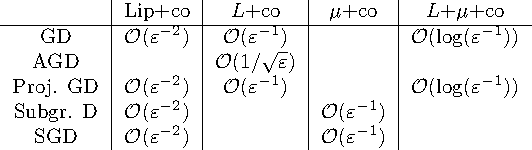
\includegraphics[width=\columnwidth]{../assets/unconstrained-cvg-table/unconstrained-cvg-table.pdf}
\end{minipage}

LMO: Let $X := \text{conv}(\mathcal{A})$, then:

\begin{minipage}{\columnwidth}
    \centering
    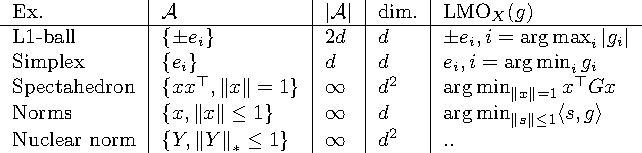
\includegraphics[width=\columnwidth]{../assets/lmo-table/lmo-table.pdf}
\end{minipage}

% Todo table for subgradient descent
Performance of AGD vs Subgr. D:

\begin{minipage}{0.8\columnwidth}
    \centering
    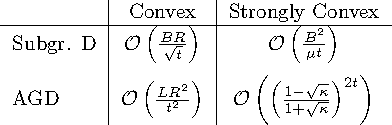
\includegraphics[width=\columnwidth]{../assets/non-smooth-subgr-table/non-smooth-subgr-table.pdf}
\end{minipage}

$\rightarrow$ Subgr. D is always slower, even in sc case only sublinear cvg.

Complexity for SGD:

\begin{minipage}{\columnwidth}
    \centering
    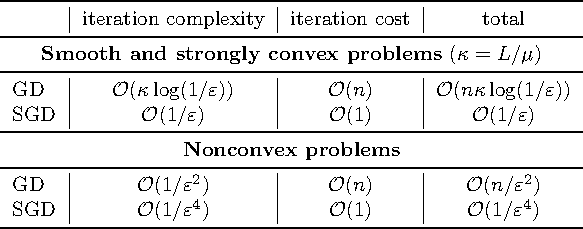
\includegraphics[width=\columnwidth]{../assets/sgd-table/sgd-table.pdf}
\end{minipage}

\textbf{Vanilla Analysis (GD \& Proj. GD):}
\begin{enumerate}
\item Use 1oc: $f(y) \geq f(x) + \nabla f(x)^\top (y-x)$
\item Set $y=x^*$, $x=x_t$: $\varepsilon_t \leq \nabla f(x_t)^\top (x_t - x^*)$
\item Use update rule: $x_t - x^* = (z_{t+1} - x^*) + \gamma \nabla f(x_t)$
    \\ where $z_{t+1} = x_{t+1}$ for GD, $z_{t+1} = y_{t+1}$ for Proj. GD
\item Apply cosine theorem: $2v^\top w = \lVert v \rVert^2 + \lVert w \rVert^2 - \lVert v-w \rVert^2$
\item For Proj. GD: Use projection property $\lVert x_{t+1} - x^* \rVert^2 \leq \lVert y_{t+1} - x^* \rVert^2$
\item Sum over $t$, telescope: $\sum_{t=0}^{T-1} \varepsilon_t \leq \frac{\gamma}{2} \sum_{t=0}^{T-1} \lVert \nabla f(x_t) \rVert^2 + \frac{1}{2\gamma} \lVert x_0 - x^* \rVert^2$
\end{enumerate}

\textbf{$L$-smooth:}
\begin{enumerate}
\item Use smoothness: $f(y) \leq f(x) + \nabla f(x)^\top (y-x) + \frac{L}{2}\lVert y-x \rVert^2$
\item Set $y=z_{t+1}$, $x=x_t$, use update rule
    \\ where $z_{t+1} = x_{t+1}$ for GD, $z_{t+1} = y_{t+1}$ for Proj. GD
\item For Proj. GD: Use projection property $f(x_{t+1}) \leq f(y_{t+1})$
\item Minimize RHS w.r.t. $\gamma$: $\gamma = 1/L$
\item Get sufficient decrease:
    \\ GD: $f(x_{t+1}) \leq f(x_t) - \frac{1}{2L} \lVert \nabla f(x_t) \rVert^2$
    \\ Proj. GD: $f(x_{t+1}) \leq f(x_t) - \frac{1}{2L} \lVert \nabla f(x_t) \rVert^2 + \frac{L}{2} \lVert y_{t+1} - x_{t+1} \rVert^2$
\end{enumerate}

\textbf{$\mu$-strongly convex:}
\begin{enumerate}
\item Use strong convexity: $f(y) \geq f(x) + \nabla f(x)^\top (y-x) + \frac{\mu}{2}\lVert y-x \rVert^2$
\item Set $y=x^*$, $x=x_t$, combine with vanilla analysis
\item Use sufficient decrease to bound/eliminate gradient term
\item For Proj. GD: Apply projection property $\lVert x_{t+1} - x^* \rVert^2 \leq \lVert y_{t+1} - x^* \rVert^2$
\item Get recursive inequality for $\lVert x_t - x^* \rVert^2$
\end{enumerate}

\textbf{Working with iterate distances:} $\lnorm x_{t+1} - x^* \rnorm^2 = \lnorm x_t - \gamma \nabla f(x_t) - x^* \rnorm^2 = \lnorm x_t - x^* \rnorm^2 - 2\gamma \nabla f(x_t)^\top (x_t - x^*) + \gamma^2 \lnorm \nabla f(x_t) \rnorm^2$ (use update rule and expand norm). Then bound middle term with $\mu$-sc and $L$-sm or similar properties. For projections in UR: use non-expansive prop.

\textbf{Telescoping sum:} $\sum_{t=0}^{T-1} (f(x_t) - f(x_{t+1})) = f(x_0) - f(x_T)$


\textbf{Matrix diff example:} 

$f(x) = \log(a^\top x) \Rightarrow \nabla f(x) = \frac{a}{a^\top x} \Rightarrow \nabla^2 f(x) = -\frac{aa^\top}{(a^\top x)^2}$ ($a_i > 0$)

$f(x) = \sum_{i=1}^d \log(x_i) \Rightarrow \nabla f(x) = ( \frac{1}{x_1}, \ldots, \frac{1}{x_d} ) \Rightarrow \nabla^2 f(x) = -\text{diag}(\frac{1}{x_1^2}, \ldots, \frac{1}{x_d^2})$

\textbf{Stochastic: } $F(x) := \E_\xi [f_\xi(x)]$. unbiased grad estimator: $\E[\nabla f_\xi(x)] = \nabla F(x)$. Then: $\nabla F(\xo) = \E[\nabla f_\xi(\xo)] = 0$. But: $\nabla f_\xi(\xo) \neq 0, \E[\Vert \nabla f_\xi(\xo) \Vert^2] \neq 0$. Jensen: $\Vert \nabla F(x) \Vert^2 = \Vert \E[\nabla f_\xi(x)] \Vert^2 \leq \E[\Vert \nabla f_\xi(x) \Vert^2]$

\textbf{Probability: } $\E[X] = \sum x_i p(x_i)$, $\text{Var}[X] = \E[(X-\E[X])^2] = \E[X^2] - \E[X]^2$, $\text{Cov}[X,Y] = \E[(X-\E[X])(Y-\E[Y])] = \E[XY] - \E[X]\E[Y]$. 

$\E[XY|Z] = \E[X|Z] \E[Y|Z]$ if $X, Y$ indep given $Z$. $P(B) = \sum P(B|A_i)P(A_i)$, $P(A|B) = \frac{P(B|A)P(A)}{P(B)}$

% todo check tables in lecture notes


    \newpage
    \section*{Newton's method}

1D: $\xtp := x_t - f'(x_t) / f''(x_t), \ t \geq 0$.

For optimization apply to $f'$: $\xtp := x_t - f'(x_t) / f''(x_t), \ t \geq 0$, resp. $\xtp := x_t - \nabla^2 f(x_t)^{-1} \nabla f(x_t)$.

$f$ co, $2\times$ diff, $\nabla^2 f(x) \succ 0$ inv, then $\xtp$ from Newton satisfies $\xtp = \argmin_{x \in \R^d} f(x_t) + \nabla f(x_t)^\top (x - x_t) + \frac{1}{2} (x - x_t)^\top \nabla^2 f(x_t) (x - x_t)$.

Let there be a ball $X \subseteq \dom(f)$ with center $\xo$ such that $\lnorm \nabla^2 f(x)^{-1} \rnorm \leq 1/\mu$ and $\lnorm \nabla^2 f(x) - \nabla^2 f(y) \rnorm \leq B \lnorm x - y \rnorm$, then for $x_t, \xtp$ resulting from a Newton step, the following holds: $\lnorm \xtp - \xo \rnorm \leq \frac{2B}{\mu} \lnorm x_t - \xo \rnorm^2$.

% TODO some other cvg theorems, not sure if relevant enough

$f$ $2\times$ diff, $\mu$-sc over open conv $X \subseteq \dom(f)$. Then $\nabla^2 f(x)$ is inv and $\lnorm \nabla^2 f(x)^{-1} \rnorm \leq 1/\mu$ for all $x \in X$.


\section*{Quasi-Newton methods}

Secant method (2nd derivative free!): Replace $f''(x)$ with $\frac{f'(x_t) - f'(\xtm)}{x_t - \xtm}$. 

% TODO skipped whole chapter for now
    \section*{Subgradient methods}

\begin{mathbox}
    {Subgradient}
    {$f: \dom(f) \to \R \cup \{+\infty\}$, co. $g \in \R^d$ is a subgradient of $f$ at $x$ if}
    {f(y) \geq f(x) + g^\top (y-x), \ \forall y \in \dom(f)}
    {Set of all subgradients at $x$ is called subdifferential $\partial f(x)$.}
\end{mathbox}

If $f$ co and diff at $x$, then $\partial f(x) = \{\nabla f(x)\}$.

$f$ co, $\dom(f)$ open, $B \in \R_+$. The following are equiv:
\begin{itemize}
    \item $\lnorm g \rnorm \leq B, \ \forall x \in \dom(f), \forall g \in \partial f(x)$.
    \item $\labs f(x) - f(y) \rabs \leq B \lnorm x - y \rnorm, \ \forall x, y \in \dom(f)$.
\end{itemize}

If $\mathbf{0} \in \partial f(x), x \in \dom(f)$, then $x$ is a \textit{global} minimum.

$f$ co, $x \in \dom(f)$. Then $\partial f(x)$ is co and closed. 

$f$ func where $\dom(f)$ is co and $\partial f(x) \neq \varnothing \ \forall x \in \dom(f)$. Then $f$ is co over $\dom(f)$. 

Directional derivatives: $f'(x;d) = \lim_{\delta \to 0^+} \frac{f(x + \delta d) - f(x)}{\delta}$. For $f$ diff $f'(x;d) = \nabla f(x)^\top d$. For subgr: $f'(x;d) = \max_{g \in \partial f(x)} g^\top d$.

\textbf{Calculating subgradients:} 
\begin{itemize}
    \item \textit{Conic combination:} $h(x) = \lambda f(x) + \mu g(x); \lambda, \mu \geq 0; f, g$ co, then $\partial h(x) = \lambda \partial f(x) + \mu \partial g(x)\ \forall x \in \text{int}(\dom(h))$.
    \item \textit{Affine compos.:} $h(x) = f(Ax + b); f$ co, then $\partial h(x) = A^\top \partial f(Ax + b)$.
    \item \textit{Supremum:} $h(x) = \sup_{\alpha \in \mathcal{A}} f_\alpha (x)$ and $f_\alpha$ co, then: $\partial h(x) \supseteq \text{conv}\{\partial f_\alpha (x) \mid \alpha \in \alpha(x)\}$ where $\alpha(x) = \{\alpha : h(x) = f_\alpha (x)\}$
    \item \textit{Superposition:} $h(x) = F(f_1(x),\dots,f_m(x))$ where $F(y_1, \dots, y_m)$ is non-decr and co, then $\partial h(x) \supseteq \left\{ \sum_{i=1}^{m} d_i \partial f_i(x) : (d_1, \dots, d_m) \in \partial F(y_1, \dots, y_m) \right\}$.
\end{itemize}


\textbf{Subgradient method:} $f$ co, possibly non-diff. Goal $\min f(x)$ s.t. $x \in X \subseteq \dom(f)$. $X$ closed+co. Let $R^2 = \max_{x,y \in X} \lnorm x - y \rnorm_2^2, B = \sup_{x,y \in X} \frac{\labs f(x) - f(y) \rabs}{\lnorm x - y \rnorm_2}$. Init $x_1 \in X$. For $t = 1, \dots, T$:
\begin{align*}
    \xtp = \Pi_X (x_t - \gamma_t g_t), \ g_t \in \partial f(x_t)
\end{align*}
For $f$ diff, this reduces to Proj GD. Subgr. Descent is not necessarily a descent method and moving along the negative direction of $g_t$ is not guaranteed to decrease the function value.

Stepsize choices:
\begin{itemize}
    \item \textit{Constant:} $\gamma_t \equiv \gamma > 0$
    \item \textit{Scaled:} $\gamma_t = \gamma / \lnorm g_t \rnorm_2$
    \item \textit{Diminishing, non-summable:} $\sum \gamma_t = \infty, \lim_{t\to\infty} \gamma_t = 0$
    \item \textit{Sq-summable:} $\sum \gamma_t = \infty, \sum \gamma_t^2 < \infty$ (e.g. $1/t$)
    \item \textit{Polyak:} Assuming $\fxo$ known. $\gamma_t = \varepsilon_t / \lnorm g_t \rnorm_2^2$
\end{itemize}

$f$ co, then SubgrD satisfies
\begin{align*}
    \min \varepsilon_t \leq \left( \sum_{t=1}^{T} \gamma_t \right)^{-1} \left( \frac{1}{2} \lnorm x_1 - \xo \rnorm_2^2 + \frac{1}{2} \sum_{t=1}^{T} \gamma_t^2 \lnorm g_t \rnorm_2^2 \right) \\
    f(\hat{x}_T) - \fxo \leq \left( \sum_{t=1}^{T} \gamma_t \right)^{-1} \left( \frac{1}{2} \lnorm x_1 - \xo \rnorm_2^2 + \frac{1}{2} \sum_{t=1}^{T} \gamma_t^2 \lnorm g_t \rnorm_2^2 \right) 
\end{align*}
where $\hat{x}_T = \left( \sum_{t=1}^{T} \gamma_t \right)^{-1} \left( \sum_{t=1}^{T} \gamma_t x_t \right) \in X$.

Using bounds $R, B$ and changing summation to $T_0 \geq 1$:
\begin{align*}
    \min_{T_0 \leq 1 \leq T} f(x_t) - \fxo \leq \frac{\frac{R^2}{2}+ \frac{1}{2}\sum_{t=T_0}^{T}\gamma_t^2 B^2}{\sum_{t=T_0}^{T} \gamma_t}
\end{align*}

% TODO: cvg results for each stepsize choice p. 219 ff

% TODO rest of chapter
    \section*{Mirror Descent}
Goal: Generalize SubgrD to non-Euclid. distances.

\begin{mathbox}
    {Bregman divergence}
    {$\omega : X \to \R$ \textit{strictly(!)} conv, continuously diff on closed conv $X$.}
    {V_\omega(x,y) = \omega(x) - \omega(y) - \nabla \omega(y)^\top (x-y)}
    {}
\end{mathbox}
$V_\omega$ is not a valid distance: asymmetric and triangle ineq. may not hold--it is called distance-generating function.

If $\omega$ $\sigma$-sc wrt some norm, then it holds $V_\omega (x,y) \geq \frac{\sigma}{2} \lnorm x - y \rnorm^2$.

For well-defined $V_\omega, V_\psi$ and $a,b > 0$ it holds $V_{a\omega + b\psi}(x,y) = aV_\omega(x,y) + bV_\psi(x,y)$.

Generalized Pythagorean: Let $\xo$ be Bregman proj of $x_0$ onto conv set $C \subset X$, $\xo = \argmin_{x \in C} V_\omega(x,x_0)$. Then for all $y \in C$: $V_\omega(y, x_0) \geq V_\omega(y, \xo) + V_\omega (\xo, x_0)$.

\textbf{Prox-mapping}: $\text{Prox}_x (\xi) = \argmin_{u\in X} \{ V_\omega (u, x) + \langle \xi, u \rangle \}$, where $\omega$ is $1$-sc wrt some norm.

\textbf{Mirror descent}:
\begin{align*}
    \xtp &= \text{Prox}_{x_t} (\gamma_t g_t) = \argmin_{x \in X} \{ V_\omega (x, x_t) + \langle \gamma_t g_t, x \rangle \} \\
    &= \argmin_{x\in X} \{ \omega (x) + \langle \gamma_t g_t - \nabla \omega (x_t), x \rangle \}
\end{align*}

Example setups
\begin{itemize}
    \item[$\ell_2$:] $X \subseteq R^n, \omega(x) = \frac{1}{2} \lnorm x \rnorm_2^2, \lnorm \cdot \rnorm = \lnorm \cdot \rnorm_2$: $V_\omega(x,y) = \frac{1}{2} \lnorm x - y \rnorm_2^2; \text{Prox}_x (\xi) = \Pi_X (x - \xi) \ \Rightarrow$ SubgrD.
    \item[$\ell_1$:] $X = \Delta_n, \omega(x) = \sum_{i=1}^{n} x_i \ln(x_i), \lnorm \cdot \rnorm = \lnorm \cdot \rnorm_1$: $V_\omega(x,y) = \sum_{i=1}^{n} x_i \ln(x_i/y_i)$ (Kullback-Leibler)$; \text{Prox}_x (\xi) = \left(\sum_{i=1}^{n} x_i \exp(-\xi_i)\right)^{-1} \begin{bmatrix} x_1 \exp(-\xi_1), \dots, x_n \exp(-\xi_n) \end{bmatrix}^\top$. Good for multiplicative updates with normalization.
\end{itemize}

\begin{smallmathbox}
    {Three point iden.}
    {\forall x,y,z \in \dom(\omega): V_\omega(x,z) = V_\omega (x,y) + V_\omega (y,z) - \langle \nabla \omega (z) - \nabla \omega (y), x-y \rangle}
\end{smallmathbox}

% Thm 11.7?


\section*{Convex conjugate}

$f: \dom(f) \to \R$, conv conj: $f^* (y) = \sup_{x\in\dom(f)} \{ x^\top y - f(x) \}$. $f$ conv is not necessary!

Fenchel inequality follows from def.: $x^\top y \leq f(x) + f^* (y)$, which is a generalization of Young's ineq $x^\top y \leq \lnorm x \rnorm^2 / 2 + \lnorm y \rnorm^2 / 2$.

If $f$ co, lower semi-continuous and proper, then $(f^*)^* = f$. That is $\lim \inf_{x\to x_0} f(x) \geq f(x_0)$ and $f(x) > -\infty$.

$f$ $\mu$-sc $\Rightarrow$ $f^*$ is $1/\mu$-Lipschitz smooth and continuously diff.

For $f, g$ proper, conv, semi-cont:
\begin{align*}
    (f+g)^* (x) &= \inf_{y} \{ f^* (y) + g^* (x-y) \} \\
    (\alpha f)^* (x) &= \alpha f^* (x/\alpha), \ \alpha > 0
\end{align*}


% ===============================

\section*{Smoothing techniques}
Goal: Approximate non-sm/diff $f$ with smooth $f_\mu$ s.t. GD and AGD can be applied.

Nesterov's smoothing: $f_\mu (x) = \max_{y \in \dom(f^*)} \{ x^\top y - f^* (y) - \mu \cdot d(y) \} = (f+\mu d)^* (x)$, where $d(y)$ is a sc, non-negative proximity function. $f_\mu$ is continuously diff and Lipschitz smooth.

Moreau-Yosida: $f_\mu (x) = \min_{y\in \dom(f)} \{ f(y) + \frac{1}{2\mu} \lnorm x - y \rnorm_2^2 \}$ for $\mu > 0$. It is equiv to Nesterov with $d(y) = \frac{1}{2} \lnorm y \rnorm_2^2$.

% TODO? Lasry-Lions, Ben-Tal-Teboulle, Randomized



\end{multicols}
\end{document}